\documentclass[pdftex, a4paper]{scrartcl}
\usepackage{ngerman}
\usepackage[utf8]{inputenc}
\usepackage[T1]{fontenc}
%\usepackage{array}
%\usepackage{subfiles}
\usepackage{url}
\usepackage[hidelinks]{hyperref}
\usepackage{parskip}
\setlength{\parskip}{1em}
\usepackage{xurl}
\usepackage[nottoc,notlot,notlof]{tocbibind}
\usepackage{longtable}
\usepackage{setspace}
\linespread{1.5}
% \usepackage[
% top    = 2.75cm,
% bottom = 2.50cm,
% left   = 3.00cm,
% right  = 2.50cm]{geometry}
\usepackage{etoolbox}
\AtBeginEnvironment{thebibliography}{\linespread{1}\selectfont}
\usepackage{endnotes}
\interfootnotelinepenalty=10000
\usepackage[acronym,toc,sort=def]{glossaries} 
\usepackage[titletoc]{appendix}
\usepackage{booktabs}
\usepackage{tabularx}
\usepackage{graphicx}
\usepackage{textcomp}
\usepackage{lscape}
\usepackage{fancyhdr} 
\usepackage{multirow}
\usepackage{caption}
\usepackage{natbib}
\usepackage[table,xcdraw]{xcolor}
\usepackage{float}
%\usepackage{lineno}
\usepackage{longtable}
\usepackage{tabularx}
\renewcommand\tabularxcolumn[1]{m{#1}}
\usepackage{enumitem}
\usepackage{spverbatim}

\makeglossaries
\loadglsentries{0.2_Glossar}

% &as_qdr=y2 (find date)

\fancypagestyle{lscape}{
\fancyhf{} %Clears the header/footer
\fancyfoot{% Footer
\makebox[\textwidth][r]{% Right
  \rlap{\hspace{1cm}% Push out of margin by \footskip
    \smash{% Remove vertical height
      \raisebox{4.87in}{% Raise vertically
        \rotatebox{90}{\thepage}}}}}}% Rotate counter-clockwise
\renewcommand{\headrulewidth}{0pt}% No header rule
\renewcommand{\footrulewidth}{0pt}% No footer rule
}

\begin{document}
  \begin{titlepage}
    \vspace*{2mm}
    \begin{center}
        \Large
        \textbf{Hochschule Worms}\\
        \textbf{Fachbereich Informatik}\\
        \textbf{Studiengang Angewandte Informatik B.Sc.}\\
        \vspace{3cm}
        \textbf{TBD}\\
        \vspace{1cm}
        \large
        Bacherloarbeit xxx\\
        \vspace{3cm}
        \begin {table}[ht]
        \centering
            \begin{tabular}{c}
                Bruno Macedo da Silva  \\ 
                676839                \\
                inf3645@hs-worms.de   \\
                Bebelstraße 22 Z10    \\
                67549 Worms            \\
            \end{tabular}
        \end {table}
        \vspace{2cm}
        \large
        \vspace{1cm}
        \begin{table}[h]
            \centering
            \begin{tabular}{l l}
                \multirow{2}{*}{Betreuer} & Prof. Dr. Zdravko Bozakov \\
                Bearbeitungszeitraum:     & Sommersemester 2023 \\
                Abgabedatum:              & xx. xxx 2023 \\
                Sperrvermerk:             & Ja/Nein \\
            \end{tabular}
        \end{table}    
    \end{center}
    \normalsize
    \vfill
\end{titlepage}
  \tableofcontents
  %\newpage
  %\addcontentsline{toc}{section}{\listfigurename}
  %\listoffigures
  \clearpage
  \printglossary[title=Glossar,toctitle=Glossar]
  \clearpage
  \newpage
  \clearpage
  \printglossary[type=acronym,title=Abkürzungen,toctitle=Abkürzungen]
  \clearpage
  \section{Einleitung}

Der heutige Netzwerkverkehr ist fast tausendfach größer als vor 20 Jahre \citep{Roser_I}. Das Internet wird heutzutage für fast all unsere Tätigkeiten verwendet: Soziale Netzwerke, Video und Audio-Streaming, Einkauf, behördliche Angelegenheiten und viele andere. So viel Verkehr generiert eine unermessliche Menge von Daten, die alle möglichen Inhalte beinhalten, von unschuldigen Anfragen nach einem eigenen Kontostand bis zur Ausführung von beabsichtigten Anfragen, um Systeme lahmzulegen. Um ersteres vom letzterem zu unterscheiden, verwenden viele Firmen das sogenannte \glsfirst*{SIEM} oder Log-Analyse-Tools. 

Das \glsfirst{NIST} definiert \gls{SIEM} als Software für die Sammlung, Anpassung, Analyse, Überwachung und Bedrohungserkennung von Sicherheitsdaten aus verschiedenen Quellen \citep{NIST_Definitions}. Die Bewertung dieser Daten spielt eine wesentliche Rolle bei solchen Anwendungen, um zu entscheiden, ob es sich um legitime Anfrage oder um einen \glsplural{Cyberangriff} handelt. Mit den Daten von \gls{SIEM} kann das \glsfirst{SOC} Team Maßnahmen ergreifen. Log Analysis und Log Management beziehen sich auf die Sammlung, Bearbeitung, Speicherung und/oder Löschen, Weiterleitung und Überwachung von Loginformationen. In dieser Arbeit benutzen wir den Begriff \quotes{Log-Analyse-Tools}, um diese Systeme zu referenzieren.

In diesem Projekt recherchieren und vergleichen wir existierende \gls{SIEM} und Log-Analyse-Tools. Danach entscheiden wir uns für eine \gls{opensource} Lösung, um eine kostengünstige Verbreitung und Implementierung zu ermöglichen. Mit dem ausgewählten Tool analysieren und bewerten wir spezifische Logdateien, damit wir demnächst potenzielle Angriffe erkennen können. Die Regelsätzen für die Angriffserkennung sollen mithilfe der \glsfirst{ttp} von \gls{mitre} aufgebaut werden.

\newpage
Unser Ziel ist es, eine umfangreiche \gls{opensource} Lösung zu finden bzw. zu gesltaten, die uns ermöglicht, \glsplural{Cyberangriff} nach vordefinierten Regelsätzen zu detektieren. \glsplural{Proprietary} Lösungen gibt es viele auf dem Markt. Sie sind meistens kostenpflichtig und verlangen spezielle Wartung. Da sich solche Lösungen eher an große Konzerne richten, beschäftigen wir uns mit dem Aufbau und Strukturierung einer eigenen Lösung mithilfe von \gls{opensource} Tools. 

Diese Arbeit wird in folgende Teile geteilt: 

% OSSIN: https://sourceforge.net/projects/os-sim/
% Preludes: https://www.prelude-siem.org/projects/prelude/wiki/ManualUser
% ELK Stack

% Grafana / Promtail: https://grafana.com/products/enterprise/
%https://grafana.com/logs/% 

%https://www.ossec.net/         https://github.com/ossec/ossec-rules

% was machen sie konkrent? / Vergleich zwischen OpenSource/Proprietary/

{\setstretch{1.5}
\begin{itemize}[noitemsep]
   \item	Definition von SIEMs und Log-Analyse-Tools 
   \item	Beschreibung von existierenden \gls{Proprietary}en und Open Source Lösungen
   \item	Entscheidung für die Implementation von einer Open Source Lösung
   \item Generierung und Extrahierung von Logdateien nach der Ausführung von einem ausgewählten \gls{Cyberangriff} 
   \item	Installation, Konfiguration und Generierung von Warnmeldungen mit den ausgewählten Anwendungen 
   \item	Definition der \gls{usecases} und Implementierung der Regelsätze für die Erkennung der vorherigen Angriffen anhand der \glsfirst{ttp} der \gls{mitre} Matrix 
   \item	Auswertung der implementierten Tools mit der Verwendung von  spezifischen Logdateien der Hochschule in der ausgewählten Lösung
\end{itemize}
}

\subsection{Problemstellung}
Während der Entwicklung dieser Arbeit beschäftigen wir uns mit folgenden Fragenstellung: 

{\setstretch{1.5}
% Regeln anhand mittre, automatisieren
\begin{itemize}[noitemsep]
   \item Wie können wir ein Log-Analyse-Tool konfigurieren, dass es vordefinierte Angriffe nach der \gls{mitre} Matrix automatisch erkennen kann? 
   \item Wie können wir allgemeine Regelsätze definieren, sodass wir sie später für die verschiedene \gls{ttp} der \gls{mitre} Matrix nanpassen können?
\end{itemize}
}

\newpage
Das folgende Diagramm, \ref{fig:AblaufderArbeit}, stellt den Aufbau und Entwicklung dieser Arbeit dar, wie oben beschrieben:
% Diagram anpassen mit korrenkten Zielen

\begin{figure}[H]
   \centering
   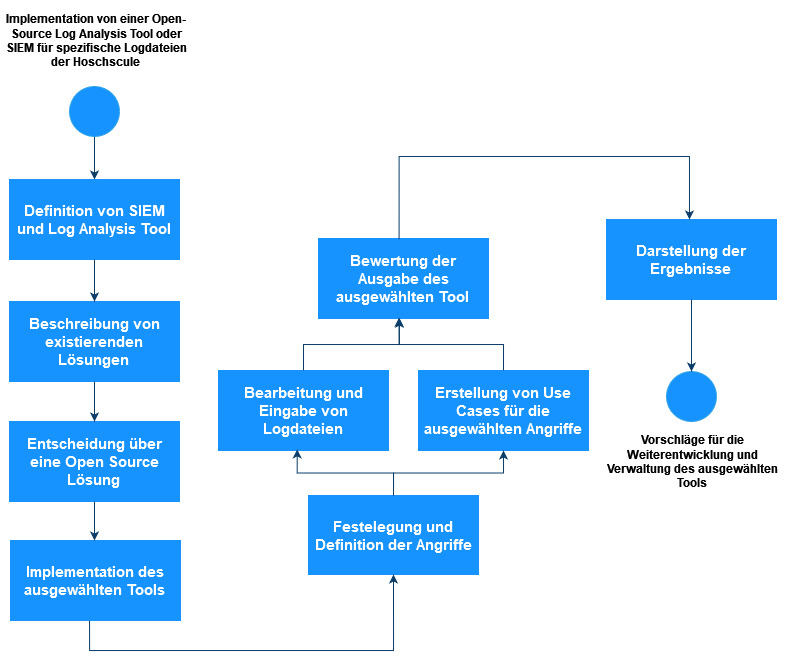
\includegraphics[width=1\textwidth]{assets/1_p1.jpg}
   \caption[Aufbau dieser wissenschaftlichen Recherche]
   {Aufbau dieser wissenschaftlichen Recherche \\Quelle: Eigene Darstellung }
   \label{fig:AblaufderArbeit}
   \centering
\end{figure}




  %\section{Anwendungsdomäne}

\begin{itemize}
    \item Theorie über Penetration Testing
    \item Theorie über Testing in Webanwendungen
    \item Art von Testen
    \item Schritte der Testing
    \begin{itemize}
        \item Strukturierung des Tests
        \item Durchführung von Testens
        \item Schlussberichtes
    \end{itemize}
\end{itemize}
  %\section{Durchführung der Aufgabe}

In diesem Kapitel beschreiben wir konkret, wie die Arbeit während meines Praxissemesters sich entwickelte. Die ersten zwei Wochen dienten als Einarbeitung und Einstieg. Nach dieser Phase bekam ich langsam und unter Betreuung mehr Verantwortung und mehr Freiheit, um die Arbeit durchzuführen. In der folgenden Tabelle wird der Ablauf systematisch und ohne Einzelheiten beschrieben. Im zweiten Teil dieses Kapitels geben wir eine ausführliche Beschreibung eines Projekts.

Jedes Projekt besitzt innerhalb von Wallsec einen festgelegten Aufbau. Dieser kann in den folgenden Punkten zusammengefasst werden:

\begin{enumerate} \label{Projektablauf}
    \item \textit{Kick-off Meeting} mit den Kunden, um grundsätzliche Informationen über die Anwendung zu bekommen
    \item Definition des Testumfangs, wie Anmeldedaten, Rolle der Nutzer, \glsplural{Tennant} und Einschränkungen
    \item Durchführung von Tests nach einer vorgegebenen Checkliste
    \item Dokumentation der durchgeführten Tests, deren gefundene \glsplural{Schwachstelle} und Vorschläge zur Härtung der Anwendung
    \item Abschlussmeeting mit den Beauftragten, um die \glsplural{Schwachstelle} und deren Ausnutzung zu präsentieren und zu demonstrieren
\end{enumerate} 

\section{Wöchentliche Zusammenfassung meines Praxissemesters}

\begin{table}[H]
    \setstretch{1.0}
    \begin{tabularx}{\textwidth}{|c|X|}
    \toprule
    \multicolumn{2}{c}{\textbf{Auflistung der Aufgabe}} \\
    \midrule
    \multicolumn{1}{c}{\textbf{Woche}} & \multicolumn{1}{c}{\textbf{Aufgabeschreibung}} \\
    \hline
    1 - 2    & Einarbeitung:
                \begin{itemize}
                    \item Installation von einer virtuellen Maschine für die Testumgebungen
                    \item Einführung in der Arbeitsablauf der Firma
                    \item Einführung, Installation und Einstellungen von \gls{burp}
                    \item Einführung in einem laufenden Projekt, um über das Ablauf- und Dokumentationsverfahren zu lernen
                    \item Durchführung und Wiederholungen von einigen Tests, um mich an den gegebenen Tools zu gewöhnen
                    \item Teilnahmen an einer Abschlussmeeting des laufenden Projekts, um das Verfahren und den Ablauf des Kundenkontakt zu erkennen und später zu wiederholen
                \end{itemize} \\
        \hline

    3 - 4       &  Start, Durchführung und Abschluss eines neuen Pentesting-Projekts an einem Versicherungsanwendung mit dem obigen beschriebenen Schritte (\ref{Projektablauf})  \\ 
    
    \hline

    5 - 6       & Weiterarbeitung an der Installation, an den Einstellungen und an der Nutzung der Tools \gls{TheHive} und \gls{Cortex}. Bereitstellung von Skripts zum Herunterladen von statistische Daten der Anwendungen und zur Automatisierung deren Nutzung.  \\ 

    \hline

    7 - 8      &  Start, Durchführung und Abschluss eines neuen Pentesting-Projekts an einer Marketing-Webanwendung mit den oben beschriebenen Schritten (\ref{Projektablauf}) \\

    \hline

    9 - 10      &  Start, Durchführung und Abschluss eines neuen Pentesting-Projekts in Netzwerk-Umgebungen mit den oben beschriebenen Schritten (\ref{Projektablauf}). Die durchgeführten Tests konzentrieren sich auf die Sicherheit eines Netzwerkes in einer Cloud-Umgebung. Für dieses Projekt spielen die Tools \gls{nmap} und \gls{scout} eine wichtige Rolle, da das Ziel war, Hosts, Dienste und dessen Einstellungen und \gls{Schwachstelle}n zu erkennen \\

    \hline

    11  	    &  Start, Durchführung und Abschluss eines Pentesting bei einer umfangreichen Webanwendung mit verschiedenen \glsplural{Tennant} und Nitzerrollen für die Verwaltung von Business-Prozessen. \\

    \hline

    11 - 14      &  Start, Durchführung und Abschluss eines Pentesting dessen Aufbau auf \glsfirst{http} und \gls{graphql} basiert. Da diese beiden Technologien mir ganz neu waren, beschäftigte ich mich intensiv damit, sie in ihrem Aufbau und in ihren möglichen \glsplural{Schwachstelle} auszukennen. \\


%    \hline

%    17 - 18      &  xxxxxx \\

%    \hline

%    19 - 20      &  xxxxxx \\


       \bottomrule
    \end{tabularx}
\end{table}

\section{Ausführliche Beschreibung eines Penetration Testing innerhalb des Praxissemesters}

Vor der Durchführung jedes Tests sind Wallsec und ihre Mitarbeiter dazu verpflichtet, eine Vertraulichkeitserklärung zu unterschreiben. Keine Informationen weder über die Firma noch über die verwendeten Methoden dürfen in irgendeiner Form veröffentlicht werden. Aus diesem Grund werden die hier demonstrierten Methoden und Tests in der Test- und Lernumgebung \glsfirst{dvwa} gezeigt. In den realen Tests verwenden wir ähnliche Methoden, manchmal mit mehr oder weniger Details, um die Sicherheit der Anwendungen zu überprüfen. 

Da dieser Bericht eingeschränkten Platz hat und dieses Thema zudem sehr umfangreich ist, demonstrieren wir in den nächsten zwei Unterkapiteln einige Methoden, die wir verwenden, um die Zielanwendung in ihrer Struktur zu kennen und auszunutzen.

\subsection{Sammlung von Informationen von dem Zielsystem}

Obwohl jede Webanwendungen ihre eigenen Eingenschaften und Ziele haben, besitzen fast alle eine ähnliche Struktur und Aufbau. Beim jedem Test fangen wir damit an, diese gemeinsame Struktur zu erkennen, indem wir nach öffentlichen Informationen suchen. Viele kritische Informationen, wie Username, Passwörter, Versionen, Systemen verbundenen IP-Adressen, lassen sich nach einer Online-Suche finden. Auch mit eingebauten Tools eines Betriebssystems können wir auf solche Informationen zugreifen. Dieses Verfahren nennen wir Banner Grabbing. Das folgende Bild zeigt ein Beispiel von einer einfachen Durchführung von Banner Grabbing:

\begin{figure}[H]
    \centering
    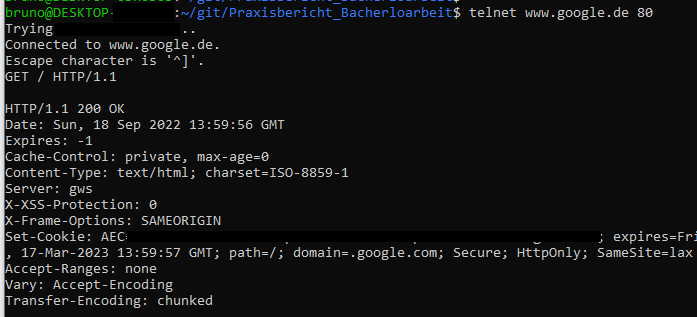
\includegraphics[width=0.5\textwidth]{/home/bruno/git/Praxisbericht_Bacherloarbeit/Praxissemester/assets/banner_grabbing.png}
    \caption{Banner Grabbing mithilfe von dem Tool telnet}
    \centering
\end{figure}

Eine Webanwendung ist eine Gruppierung von verschiedene Verzeichnissen. Jedes Verzeichnis soll dem Nutzer eine Information oder Interaktion anbieten. Manche sind aber nicht für Nutzer gedacht und dienen zur Verwaltung von Einstellungen. Da solche Verzeichnisse nicht direkt aufrufbar sind  benutzen wir als Tester andere Methode, um zu finden, was die Entwickler im Hintergrund beibehalten wollen. Es gibt verschiedene Tools, die mithilfe von sogenannten \textit{wordlists}, viele Anfragen an eine Anwendung schicken, um herauszufinden, was nicht direkt von dem Browser aufrufbar ist. Solche \textit{wordlists} sind Textdateien, die häufig verwendete Wörter beinhalten, die für Webanwendungen, Nutzername oder Passwörter verwendet werden. Da viele Webanwendungen ähnliche Strukturen haben, wird auch meistens erwartet, dass gewöhnliche Wörter auch zu finden sind. Das nächste Beispiel zeigt uns, dieses Entdeckungsverfahren auf unserem Ziel, \gls{dvwa} Tool. Hier benutzen wir das Tool \gls{dirb}, um herauszufinden, welche Verzeichnisse in dieser Anwendung existieren. In diesem Fall werden verschiedene Anfragen geschickt, jede mit einem verschiedenen Wort, um zu sehen, welche positive Antworten liefern. Das folgende Bild zeigt die Durchführung und das Ergebnis des Scanverfahrens mithilfe des Tools \gls{dirb}:

\begin{figure}[H]
    \centering
    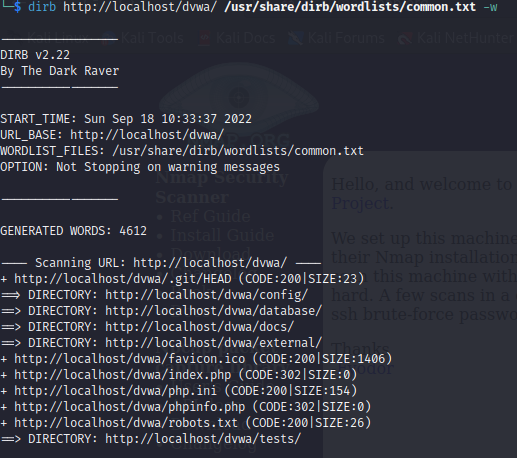
\includegraphics[width=0.5\textwidth]{/home/bruno/git/Praxisbericht_Bacherloarbeit/Praxissemester/assets/dirb.png}
    \caption{Brute force Scan für Verzeichnisentdeckung}
    \centering
\end{figure}

Der nächste Schritte wäre eine manuelle Beobachtung des entdeckten Materials, um zu finden, ob irgendwelche sensitiven Information ausgeliefert wurde. Falls ja, würden wir dann versuchen diese \gls{Schwachstelle}, zu erkennen und auszunutzen.

Ein Netzwerk-Scan ist auch eine häufig verwendete Methode, um Dienste innerhalb des zu testenden Objekts zu finden. Dieser Scan schickt an das Ziel verschiedene Anfragen, damit wir die Reaktion des Zielsystems beobachten können. Während wir uns bei dem ersten Scan auf die Webanwendung fokussierten, bearbeiten wir hier eine Ebene, die nicht für die normale Nutzung gedacht ist. Unser Fokus liegt auf dem Server, wo die Anwendung läuft. Dafür testen wir die sogenannten \gls{port}. Aus diesem Scan lassen sich meistens viele nützliche Informationen herausfiltern, wie Betriebssystems, wo die Webanwendung läuft, Name und Versionen der existierenden Dienste. Mit diesen Informationen ist es möglich dann zielgerichtete Angriffe vorzubereiten, um \glsplural{Schwachstelle} auszunutzen.

Das nächste Bild zeigt das Ergebnis der Durchführung von \gls{nmap} gegen das Testziel \textit{scanme.nmap.org}:

\begin{figure}[H]
    \centering
    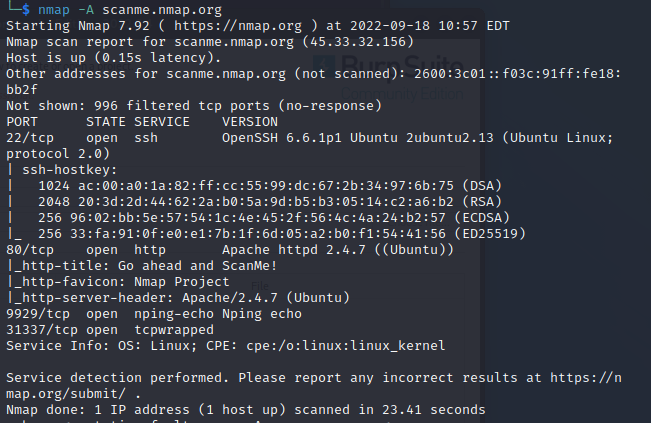
\includegraphics[width=0.5\textwidth]{/home/bruno/git/Praxisbericht_Bacherloarbeit/Praxissemester/assets/nmap.png}
    \caption{Brute force Scan für Verzeichnisentdeckung}
    \centering
\end{figure}

Aus diesem Scan erfahren wir welches Betriebssystem und welche Version die Webanwendung benutzt. Auch wenn solche Versionen gegen Angriffe geschützt sind, ist es unsere Aufgabe den Kunden zu informieren, dass sensitive Informationen für alle sichtbar sind. Ein bösartiger Nutzer könnte diese Informationen nutzen, um eine \glsplural{Schwachstelle} für diese Anwendungen zu finden und dann auszunutzen.

\subsection{Ausnutzung der Zielanwendung}

Nachdem die vorherigen Scans durchgeführt wurden und öffentliche Serverseite Informationen gesammelt wurden, fangen wir mit den Tests auf der Webanwendung an. In diesem Fall ist es unser Ziel zu wissen, welche versteckten Daten oder unerlaubten Aktionen ein Angreifer durchführen kann, um die \gls{CIA} der Anwendung zu verletzen. Für die folgenden Tests benutzen wir unter anderen auch das Tool \gls{burp}.

Unser erster Test soll überprüfen, ob es möglich ist, in ein Eingabefeld Daten einzutragen und das normale Verhalten der Anwendung zu ändern. Wir wollen eigenen Code hinzuführen und in dem Falle, dass es uns gelingt, das zu tun, können wir dann weiteren Code hinzufügen, um Daten von Nutzer zu stehlen oder das normale Verhalten der Anwendung beschädigen. Wir prüfen hier, ob die Anwendung gegen \glsfirst{xss} anfällig ist. Um diesen Test durchzuführen, fügen wir erwartete Daten hinzu, um das Verhalten der Anwendung zu beobachten. Nachdem wir das normale Verhalten erkannt haben, versuchen wir eigenen Code hinzufügen und beobachten, ob wir die Anwendung ausnutzen können. 

\begin{figure}[H]
    \centering
    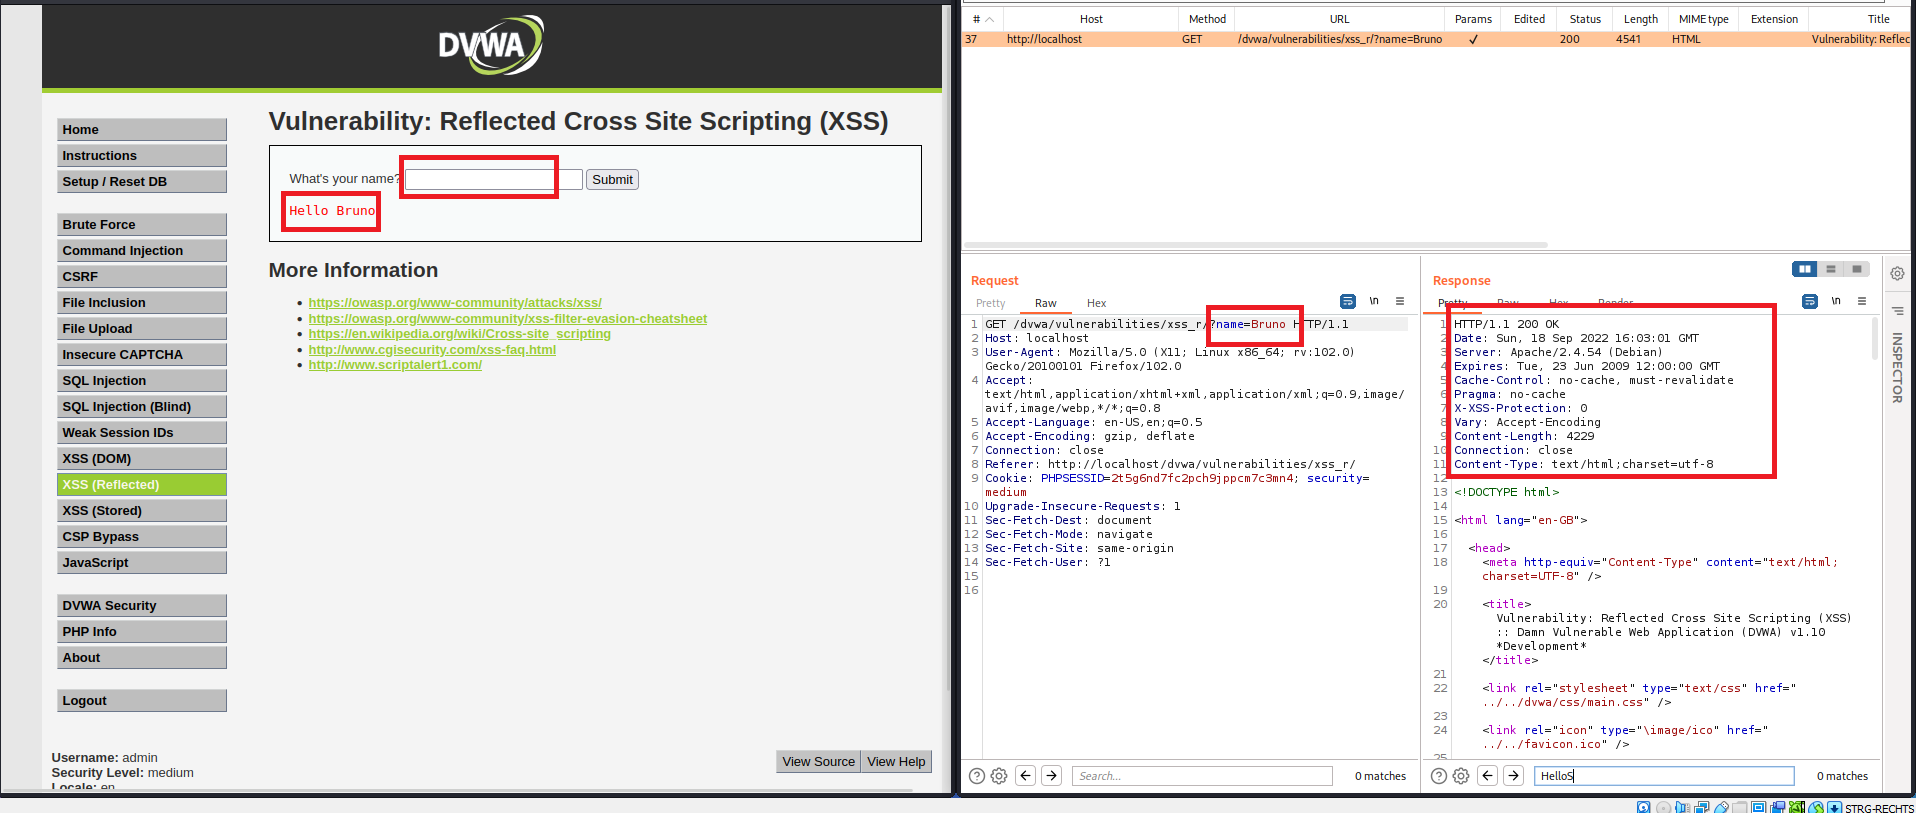
\includegraphics[width=0.8\textwidth]{/home/bruno/git/Praxisbericht_Bacherloarbeit/Praxissemester/assets/xssnormal.png}
    \caption{Beobachtung der Anwendung unter normale Nutzung}
    \label{fig:xssnormal}
    \centering
\end{figure}

Das Bild \ref{fig:xssnormal} zeigt den ersten Test. Aus dieser Aufnahme der Anfrage können wir sehen, dass die Nutzereingabe direkt in dem Browser stattfindet. Wir sehen in der Antwort Informationen über den Aufbau der Anwendung und wie sie auf unsere Anfrage reagiert. Auf dem nächsten Bild versuchten wir bösartigen Code hinzuzufügen, um den normalen Ablauf der Anwendung zu verletzten. Dafür verwenden wir \gls{javascript} Code. Wir können unseren Code direkt in die Anwendung, in einen selbst gebastelte Request oder in \gls{burp} eingeben:

\begin{figure}[H]
    \centering
    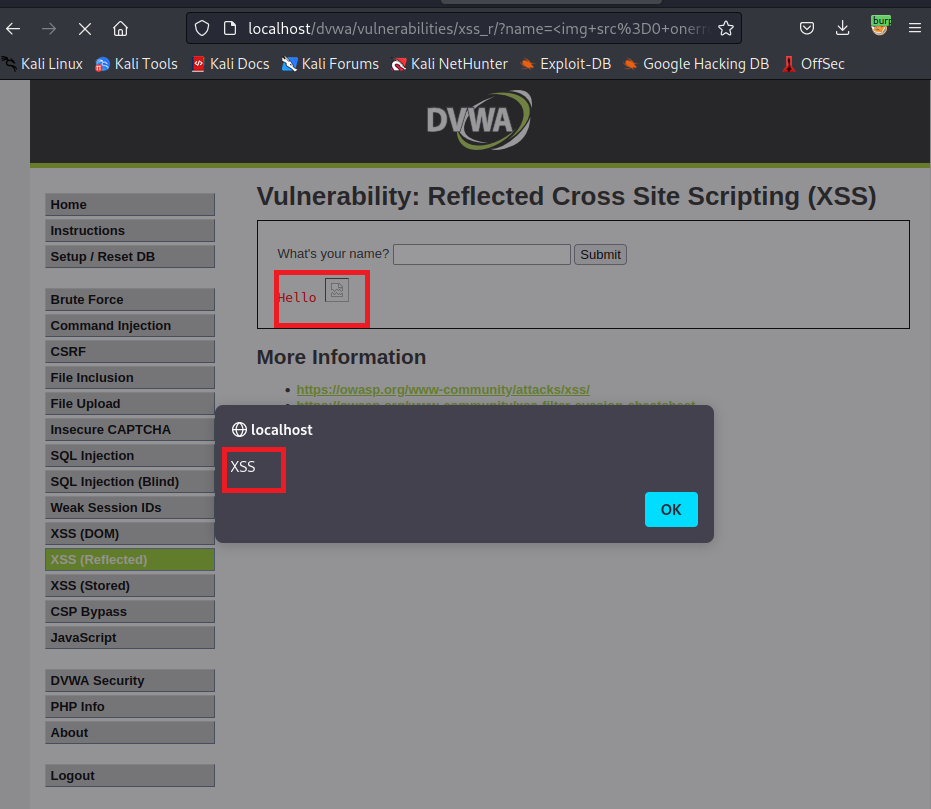
\includegraphics[width=0.8\textwidth]{/home/bruno/git/Praxisbericht_Bacherloarbeit/Praxissemester/assets/xss.png}
    \caption{Einführung von bösartigen Code und Beobachtung der Reaktion der Anwendung.}
    \label{fig:xssexecuted}
    \centering
\end{figure}

Für diesen Test haben wir den Code \textit{<img src=0 onerror='alert(``XXS'')'\textbackslash>} hinzugefügt. Das Ziel dieses Codes ist ein nicht existierendes Bild hinzuzufügen, um einen absichtlichen Fehler zu provozieren. Dieser Fehler zeigt ein kleines Fenster in der Anwendung mit dem Text ```XSS'''. Eine geschützte Anwendung würde entweder den Code und ihren Zeichen ``< >'' ignorieren oder diese zu anderen übersetzen. Es kann auch sein, dass die Anwendung dem Nutzer sagt, dass die eingegebenen Zeichen nicht erlaubt nicht. Aus dem Bild sehen wir aber, dass die Anwendung alle Zeichen akzeptiert und sogar erlaubt, dass der Code ausgeführt wird. Aus dieser Situation hätten wir einen \glsfirst{pof}, dass die Anwendung gegen diese Art von Angriff anfällig ist.


\subsection{Kundebericht}

Je nachdem wie lange das Projekt läuft, können wir mehr oder weniger zeitintensive Tests durchführen. Am Ende des Projekts präsentieren wir dem Beauftragten in einem Meeting unser Ergebnis und liefern ein Bericht mit detaillierten Informationen über die gefundenen \glsplural{Schwachstelle} und die dazu verwendeten Methoden, um sie zu finden. Dieser Bericht wird so geschrieben, damit non-native Nutzer es verstehen können. 

In den ersten Abschnitten erklären wir mit weniger technischen Begriffen, wie und was für Tests durchgeführt wurden. In den folgenden Kapitel erklären wir mit mehr Einzelheiten und technischen Details, wie wir zu unserem Ergebnis kamen. Anschließend geben wir Vorschläge für die Verbesserung der Sicherheit der Webanwendung und am Ende geben wir mithilfe von \gls{CVSS} oder von den Kunden ausgewählten Metrik eine allgemeine Bewertung.

  %\section{Fazit}

\subsection{Diskussion der Ergebnisse}
In dieser Arbeit emulierten wir, mithilfe von Grafana, Loki und Promtail eine \gls{SIEM}-Lösung, um Überwachungsmechanismen anhand von Logdateien zu erstellen. In der Tabelle \ref{tab:VerewendeteTools} zeigen wir die Rolle jedes verwendeten Tools bei der Erreichung unseres Ziels:

\begin{table}[h]
    \centering
    \setstretch{1.2}
    \begin{tabular}{|c|c|}
    \hline
    \textbf{Tool}    & \textbf{Funktionalität}         \\ \hline
    Promtail         & Datensammlung                   \\ \hline
    Loki             & Normalisierung und Vearbeitung  \\ \hline
    Grafana          & Berichts- und Grafikgenerierung \\ \hline
    Grafana:Alerting & Generierung von Warnmeldungen   \\ \hline
    \end{tabular}
    \caption{Verwendete Tools und ihre Hauptfunktionalitäten} 
    {Verwendete Tools und ihre Hauptfunktionalitäten}
    \label{tab:VerewendeteTools}
\end{table}

Wir stellen fest, dass die verwendeten Tools eine kosteneffektive Möglichkeit bieten, ein Überwachungssystem zu implementieren. Die Methoden zur Erkennung von Angriffen lassen sich anhand der \glsfirst{ttp} der \gls{mitre} Matrix definieren. Nach der Auswahl eines Angriffs erstellen wir Regelsätze mit der Abfragesprache \gls{logql} in Loki, um Muster zu identifizieren, die auf den ausgewählten Angriff hindeuten. Diese Regelsätze werden dann verwendet, um Warnmeldungen über den Angriff zu generieren und zu versenden.

Zu unsere initialen Ziele:

{\setstretch{1.5}
\begin{itemize}[noitemsep]
   \item Wie können wir ein Log-Analyse-Tool konfigurieren, dass es vordefinierte Angriffe nach der \gls{mitre} Matrix automatisch erkennen kann? 
   \item Wie können wir allgemeine Regelsätze definieren, sodass wir sie später für die verschiedene \gls{ttp} der \gls{mitre} Matrix anpassen können?
\end{itemize}
}

können wir sagen, dass die \gls{mitre} Matrix umfangreiche Informationen anbietet, um präzise Regelsätze zu generieren. 

\subsection{Herausforderungen}
Zu unserem primären Ziel können wir sagen, dass die \gls{mitre}-Matrix umfangreiche Informationen bietet, um zielgerichtete Regelsätze zu generieren. Die Erstellung dieser Regelsätze kann jedoch eine der größten Herausforderungen bei der Implementierung darstellen, da die Verwendung der Abfragesprache \gls{logql} viel Zeit in Anspruch nehmen kann. Sobald diese Hürde jedoch überwunden ist, ist es möglich, präzise Regelsätze zu erstellen, um potenzielle Angriffe zu identifizieren. Die Lernkurve für den Aufbau der richtigen Regelsätze kann eine große Herausforderung darstellen, wie auch in unserem Fall.

Da Logdateien aus produktiven Umgebungen eine große Menge an Informationen enthalten, müssen die Regelsätze so definiert werden, dass sie die relevanten Informationen wie IP-Adresse, Portnummer, Zeitfenster und Zeitabstände zwischen Anfragen filtern und nach Angriffsmustern kategorisieren können.

Die zweite große Herausforderung bestand darin, die richtigen Einstellungen und Funktionen von Promtail, Loki und Grafana zu verwenden. Das Beherrschen dieser Elemente kann dazu beitragen, dass die Anwendungen reibungslos funktionieren und vertrauenswürdige Ergebnisse liefern.

Die korrekte Konfigurierung von Promtail, besonders von \quotes{scrape\_configs}, begünstigt die Extrahierung spezifischer Informationen und die Generierung präziser \quotes{Labels}. Das Verständnis über die vielfältigen Funktionalitäten von Grafana trägt dazu bei, dass die ausgegebenen Daten die notwendigen Informationen enthalten, um den Entscheidungsprozess zu erleichtern. Die richtigen Einstellungen gewährleisten eine fehlerfreie Nutzung der Anwendungen und erleichtert ihre Skalierbarkeit. In diesem Fall können sowohl die offizielle Dokumentation als auch die offiziellen Forenbeiträge dazu beitragen, die Tools richtig zu konfigurieren.

\newpage
Letztendlich sind \quotes{Labels} wichtige Elemente bei Grafana, Loki und Promtail. Die richtige Indizierung spielt eine entscheidende Rolle für die Leistung der Anwendung. Die Verwendung vieler \quotes{Labels} erfordert hohe Rechenkapazität und kann auch zu fehlerhaften Ergebnissen führen. Die Rechenkapazität muss ebenfalls angepasst werden, um Abstürzen wegen steigenden Anfragen (siehe Abbildung \ref{fig:Eskalation_Labels} auf Seite \pageref{fig:Eskalation_Labels}) zu vermeiden.

\subsection{Zukünftige Forschung}
Dieser Arbeit ermöglicht eine Weiterentwicklugn in verschiedenen Bereichen:
 
\begin{itemize}[noitemsep]
    \item \textbf{Abdeckung vielen möglichen \glsplural{Cyberangriff}n mit neuen Regelsätze und Dashboards}:
\end{itemize}

Mit der Nutzung der \glsfirst{ttp} der \gls{mitre} Matrix ist es möglich, Regelsätze in \gls{logql} für andere \glsplural{Cyberangriff} aufzubauen und dadurch Logdateien aus verschiedenen Systemen und Anwendungen zu verwenden. Mit anderen Regelsätzen ist es möglich umfassende Sicherheit für produktive Umgebungen zu bieten, indem mehr \glsplural{usecases} abgedeckt werden, um Angriffe zu erkennen. Zur Unterstützung bietet Grafana in ihrer offizielen Webseite bereits kundenspezifische Dashboards an, die verwendet und an die jeweilige Situation angepasst werden können.

\begin{itemize}[noitemsep]
    \item \textbf{Beherschung der Tools: Promtail, Loki und Grafana}:
\end{itemize}

Grafana, Loki und Promtail bieten in ihrer Konfiguration verschiedenen Möglichkeiten, um Informationen von Logdateien zu extrahieren, zu filtern und zu analysieren. Eine tiefe Beherrschung von \quotes{scrape\_configs} von Promtail trägt dazu bei, Logdateien zu erkennen und wichtige Informtionen direkt zu filtern, ohne das weitere Abfragen notwendig sind, indem auch Leistung gespart wird. Eine Weiterarbeit mit der \gls{abfragesprache} \gls{logql} hilft dabei, präzise und effizieren Abfrage aufzubauen, um bessere Grafiken und/oder Warnmeldung zu genieren. Zusätzlich kann die vielfältigen Funktionalitäten von Grafana dabei unterstützen, zuverlässige Grafiken und Tabellen zu generieren, um nützliche Informationen aus den Logdateien grafisch darzustellen. Die Beherrschung dieses Tool stellt auch eine mögliche und vielversprechende weitere Recherche dar. 


\begin{itemize}[noitemsep]
    \item \textbf{Umfangreiche Beobachtbarkeit mit den Tools der \textit{\gls{GrafanaSystem}}}:
\end{itemize}

Die Tools um den \textit{\gls{GrafanaSystem}} bieten viele Möglichkeiten, um eine deutliche und akkurate Beobachtbarkeit eines Systems durchzuführen. Wenn kombiniert, ermöglichen sie eine holistische Analyse von \gls{pillarobservability}. Die kombinierte Implementierung in einer produktiven Umgebung kann dazu beitragen, die Sicherheit eines Systems auch bei skalierbaren Umgebungen zu verbessern. Eine Recherche in dieser Richtung hat auch die Möglichkeit, positive Ergebnisse zu liefern.


\begin{itemize}[noitemsep]
    \item \textbf{Automatische Antworten auf mögliche \glsplural{Cyberangriff}n}:
\end{itemize}

Eine umfangreiche \gls{SIEM}-Lösung bietet laut \cite{Mohammed_NOC} die wichtigsten Informatinen, um Angriffe zu erkennen. Die Sicherheitsanalyse stoppt jedoch nicht in der Erkennung, sondern verlangt Handlungen, um laufende Angriffe zu stoppen oder potenzielle zu verhindern. Die Entwicklung oder die Integration von existierenden Tools, um automatisch gegen \glsplural{Cyberangriff} zu handeln, stellen auch eine mögliche Perspektive für zukünftige Recherche dar.

\begin{itemize}[noitemsep]
    \item \textbf{Nutzung von \gls{KI}}:
\end{itemize}

Moderne Angriffe haben heutzutage einen dynamischen Aspekt, der sich an die Umgebung anpasst, insbesondere durch die fortschreitende Entwicklung von \glsfirst{KI} \citep{Guembe_AIHACKER}. \gls{KI} kann zur Automatisierung von Aufgaben oder zur effizienten Datenanalyse eingesetzt werden. Für die Weiterentwicklung dieser Arbeit kann \gls{KI} eine Unterstützung bei dem Aufbau von performanteren Regelsätzen bieten, um zuverlässiger und effizienter Log-Analyse zu gestalten.

Diese Möglichkeiten zusammen oder getrennt könnten dazu beitragen, einen sicheren Netzwerkverkehr zu gewährleisten.

  \nocite{*}
  \begingroup
    \setlength{\bibsep}{4pt}
    \setstretch{1}
    \bibliography{7_Referenzen}
    \endgroup
  \bibliographystyle{apalike}
 % \setcitestyle{authoryear, open={\(},close={\)}
  %\newpage
    
\end{document}


% &as_qdr=y2